\subsection{Memory Resistor}

In 2008, a group of researchers from HP labs published a paper entitled \textit{``The missing memristor found''} \cite{hp_memristor_found}. What, then, is a memristor, and how did we know it was missing? A memristor (short for memory resistor) is a resistor with memory whose resistance depends on the past flows of current passed through the circuit. The resistance of a memristor is increased by current travelling through it in one direction, and decreased by current travelling through it in the other direction. A memristor is a passive circuit which remembers its resistance even when inactive and without power for long periods of time. These properties make memristors interesting candidates for non-volatile storage and memory units, as they retain their state when unpowered, and specifically as they enable storage of continuous ranges of values (i.e. low \textit{through} high resistance) in contrast to discrete binary values (i.e. 0 \textit{or} 1) \cite{memristors_a_new_frontier}.

Back in 1971, Leon Chua, often referred to as the father of non-linear circuit theory, laid the mathematical foundation detailing the relations between the four fundamental circuit elements. Interestingly, at that time only three fundamental circuit elements had physical counterparts, namely resistors, capacitors and inductors. The fourth fundamental circuit element, the memristor, was only conceptualized in theory by Chua for the sake of symmetry (see figure \ref{fig:circuit_elements}). As outlined in Chua's seminal paper \textit{``Memristor-the missing circuit element''} \cite{chua_memristor}, the current-$I$ voltage-$V$ curve of a memristor has a unique shape, an IV-fingerprint if you will, in the form of a pinched hysteresis loop (see figure \ref{fig:pinched_hysteresis}). A hysteresis loop indicates that a system has an internal state (i.e. memory) which affects the output of the system and which depends on past inputs to the system \cite{memristor_hayes}. As famously state by Chua, \textit{``If it's pinched it's a memristor''} indicates that the hysteresis loop of a memristor passes through the origin.

\begin{figure}[htbp]
	\begin{center}
		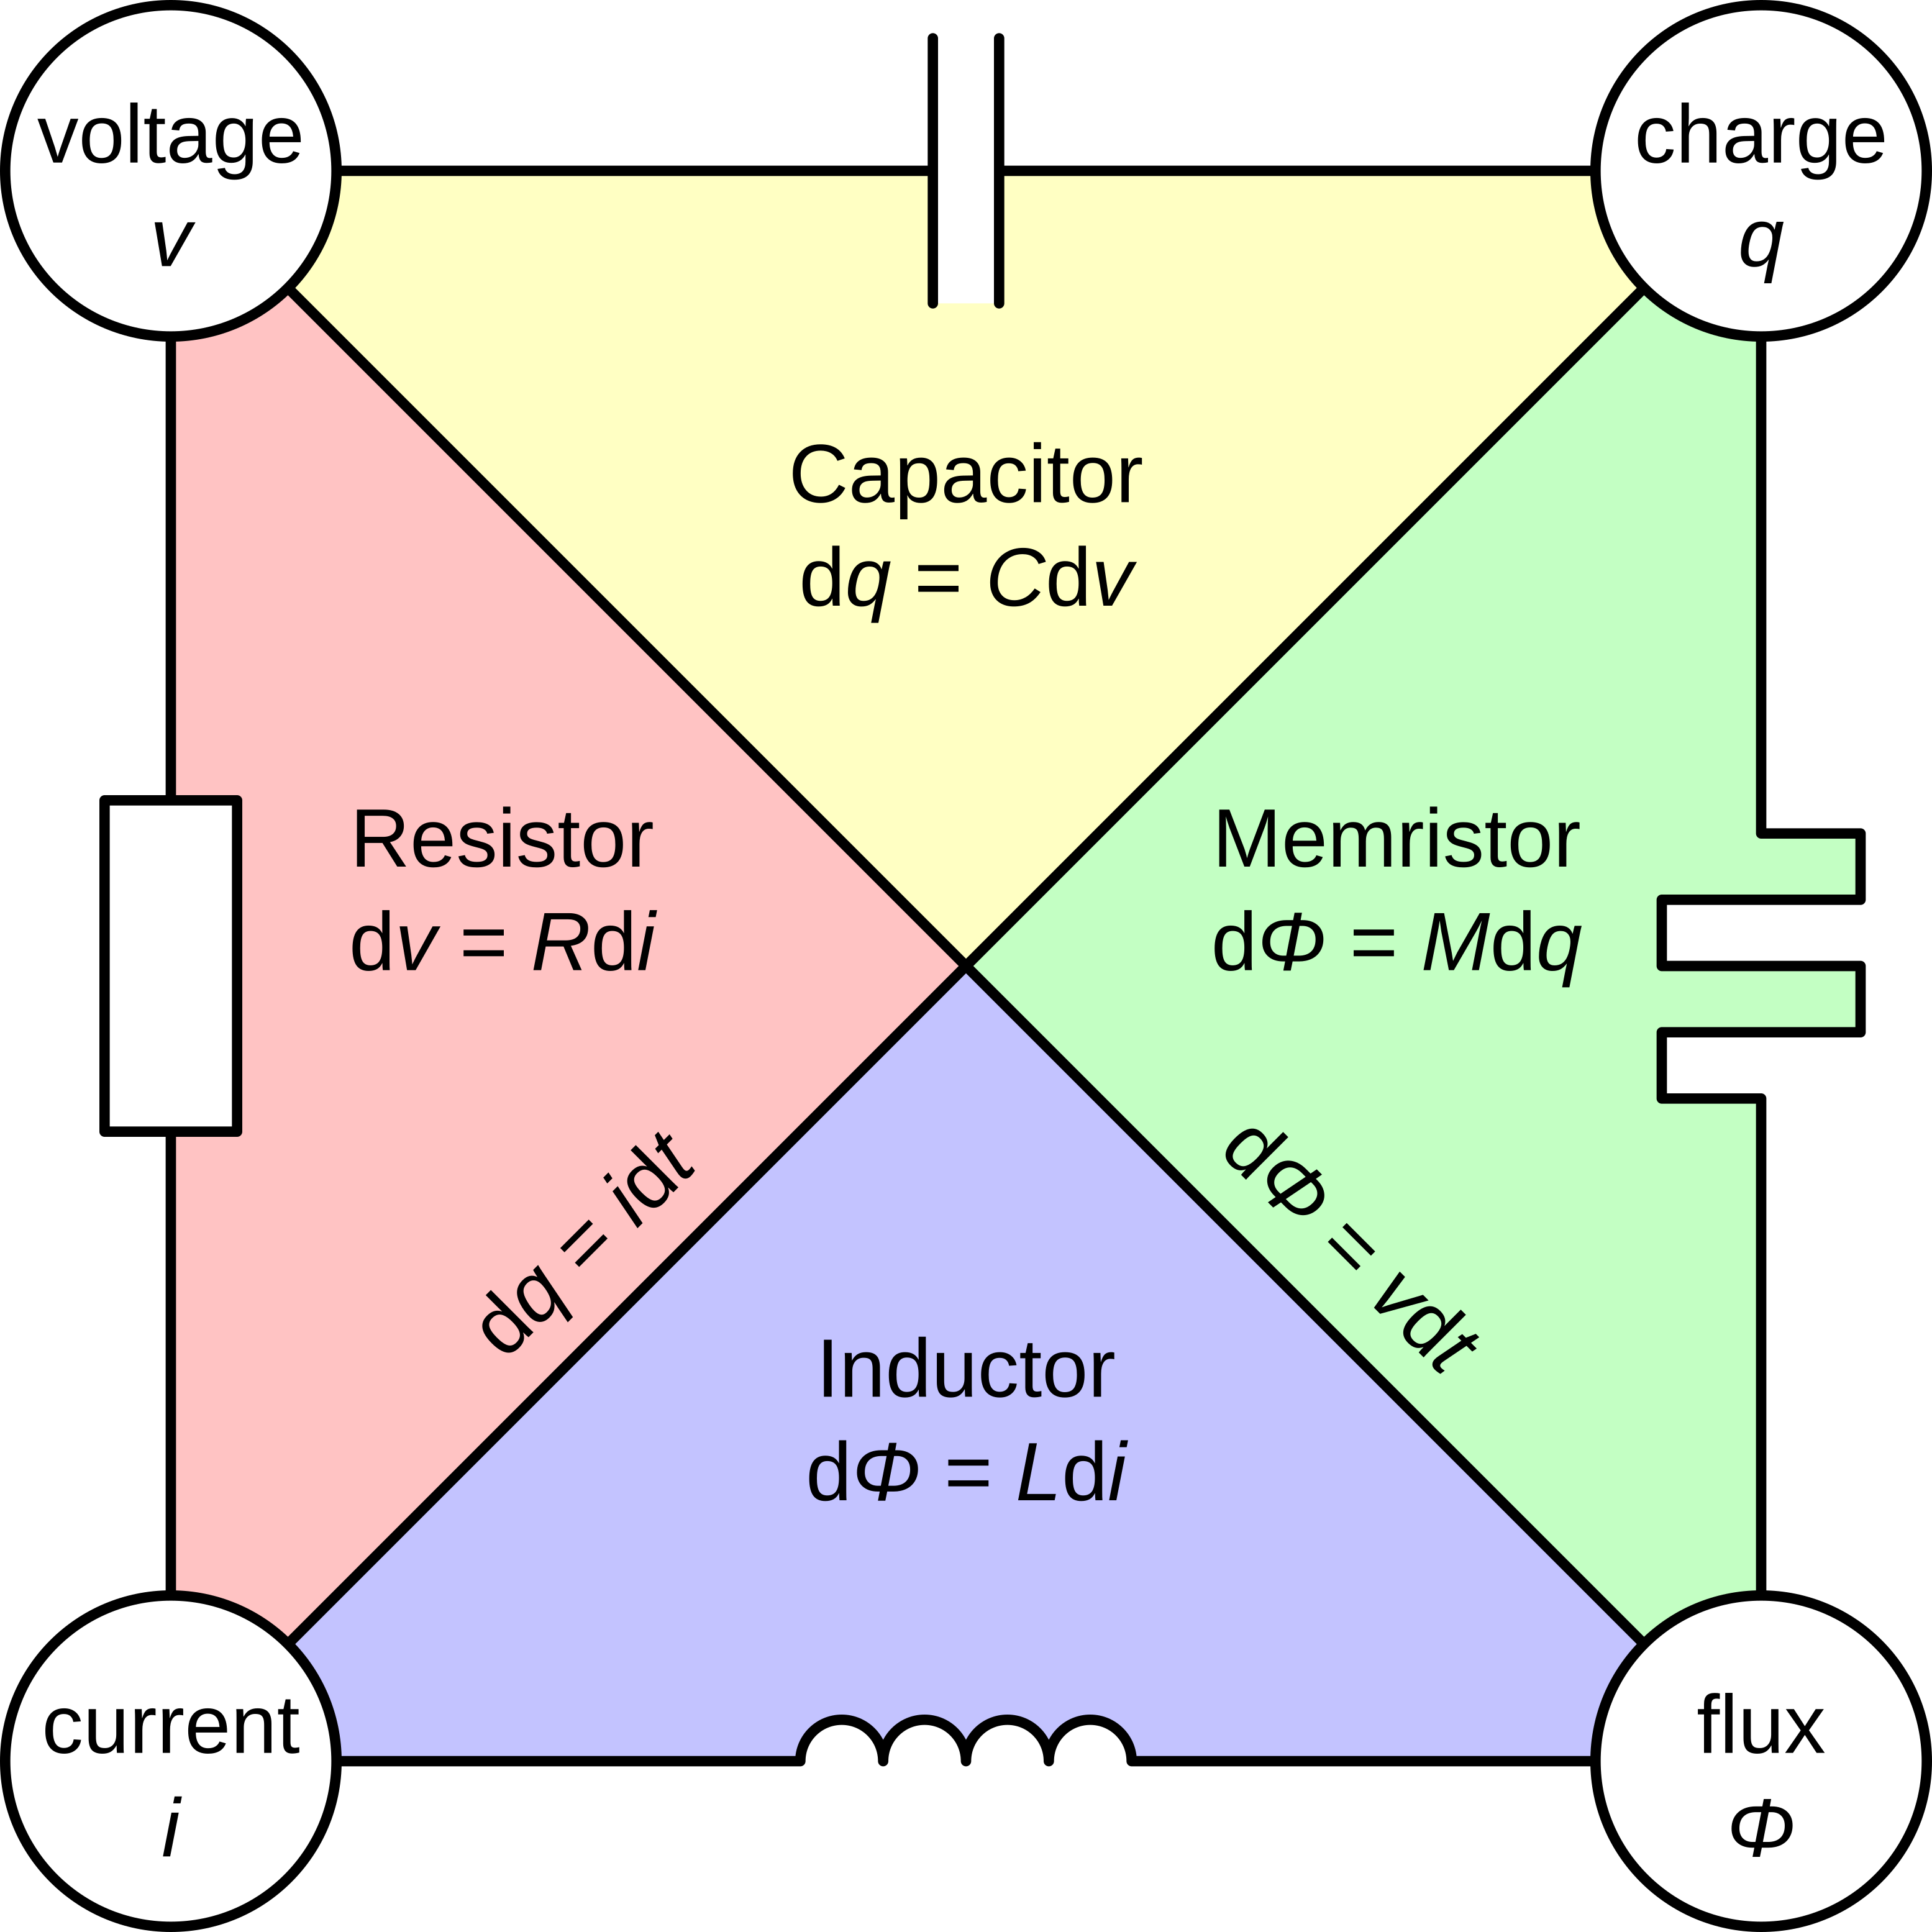
\includegraphics[width=0.5\textwidth]{inc/circuit_elements.png}
		\caption{Fundamental circuit elements.\protect\footnotemark}
		\label{fig:circuit_elements}
	\end{center}
\end{figure}
\footnotetext{Original image (CC BY-SA): \url{https://en.wikipedia.org/wiki/File:Two-terminal_non-linear_circuit_elements.svg}}

\begin{figure}[htbp]
	\begin{center}
		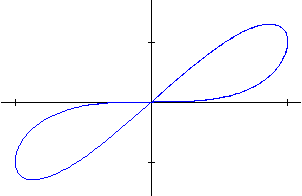
\includegraphics[width=0.5\textwidth]{inc/pinched_hysteresis.png}
		\caption{IV-curve of a memristor circuit, arrow indicates time.\protect\footnotemark}
		\label{fig:pinched_hysteresis}
	\end{center}
\end{figure}
\footnotetext{Original image (© Brian Hayes): \url{https://www.americanscientist.org/libraries/documents/201128120228377-2011-03CompScienceHayes.pdf}}

Ever since 2008, there has been an exponential increase in research related to memristors, where the number of search results for ``memristor'' on Google Scholar has doubled every 18-24 months \cite{memristors_a_new_frontier}. Why are so many researchers attracted to this new field, and what motivates such a profound investment of time and resources into this research?

% ref: Tim Molter HiPeac Prague 2016 Memristor Keynote
%
% Denser memory, faster read and write, lower energy use, non-volatile, and may represent continuous (i.e. not 0 and 1).

% ref: Tim Molter HiPeac Prague 2016 Memristor Keynote
%
% 1 billion fold discrepancy between current machine learning platforms and biological brains.
%
% We can operate on very low voltages because of the read and write phases that constantly repair relevant state.

% === [ Subsections ] ==========================================================

\subsubsection{Artificial Synapses}

% TODO: Continue from here.

Several similarities have been identified between the properties of memristors and synapses, which make them interesting candidates for associative memory models; as further described in section \ref{sec:current_capabilities_memory_resistor}.

% TODO: Merge the contents of the following input files into this file, when they have matured, and remove the respective input files.

% NOTE:
% * Key idea: memory access is adaptation is processing.
%
% ref: https://www.youtube.com/watch?v=CFSrC7kjbJo ("Introduction to AHaH Computing, Alex Nugent, RIT, April 2015")

% +--- New paradigm
% |
% V

% ref: http://knowm.org/
%
% > ## New paradigm of computing
% >
% > The act of accessing memory is the act of processing.

% +--- Key point!
% |
% V

% ref: https://www.youtube.com/watch?v=CFSrC7kjbJo ("Introduction to AHaH
%
% > XXX [ IMPORTANT ] XXX
% >
% > Synaptic access is processing is adaptation (memory and processing merged, d=0).
% >
% > XXX [/ IMPROTANT ] XXX


% NOTE:
% * distance between memory access and processing is 0 in the brain, which has a tremendous impact on the energy efficiency of highly adaptive systems.
%
% ref: https://www.youtube.com/watch?v=CFSrC7kjbJo ("Introduction to AHaH Computing, Alex Nugent, RIT, April 2015")

% +--- motivation behind AHaH nodes and new paradigm of computing.
% |
% V

% ref: http://knowm.org/knowm-api/
%
% Every modern computing system currently separates memory and processing. This works well for many tasks, but it fails for large-scale adaptive systems like brains or large ML models like neural networks. Indeed, there is no system in Nature outside of modern human digital computers that actually separates memory and processing, so it’s a wonder we have been able to do as much as we have.

% ref: http://knowm.org/
%
% > ## Modern computing
% >
% > Clear distinction between memory and processing.
% > Shuttle information back and forth.
% > Takes too long, requires too much energy.

% ref: https://www.youtube.com/watch?v=Tb2E-t11OH4 ("What is AHaH Computing?")
%
% > Large scale adaptive learning systems, like brains.
% >
% > Bring memory and processing closer together. Parallel computing.
% >
% > Reduce or eliminate the energy normally associated with computing those functions.

% ref: https://www.youtube.com/watch?v=R7HxFhVQVr4 ("Why AHaH computing?")
%
% > Current digital computing platforms are billions of times less power and space efficient than biology (brains) for synaptic operations.
% >
% > It's physically not possible to reach biological level efficiency without significant changes in both architecture and technology.
% >
% > "GPU's will save us." `No they won't, they just suck less`
% >
% > If you insist on separating memory and computing, you won't even get close to the capacity of biology.
% >
% > Traditional computing would go an inch while biology is able to circle the world.


% NOTE:
% * Points of bifurcation, forks in the road, branches. Two memristors. Difference in resistance determine the value of the synapse.
% * Energy dissipating pathways. Fractal patterns.
%
% ref: https://www.youtube.com/watch?v=CFSrC7kjbJo ("Introduction to AHaH Computing, Alex Nugent, RIT, April 2015")

% +--- Synapse consists of two memristors, competing.
% |
% V

% ref: https://www.youtube.com/watch?v=IVDRcV8XvlI ("What is an AHaH node?")
%
% > Two memristors competing with each other.
% >
% > A kT-bit (thermodynamic bit), a synapse consisting of two memristors.
% >
% > Look at the leaf of a plant. Energy dissipating system, constructed of many bifurcating channels. Every place where the energy flow splits, you have an AHaH node. You have two competing energy dissipating pathways.
% >
% > Nature is built of AHaH nodes.
% >
% > Understand how things self-organize.

% ref: http://knowm.org/knowm/
%
% A memristor is the electronic equivalent of an adaptive container!
%
% “Knowm's Synapse” or “Nature’s Transistor”. Two competing energy dissipation pathways.
%
% As a voltage (pressure) is applied to a memristor, its conductance will change.
%
% It is responsible for most self-organization on this planet. Nature is built of Knowms, including you.
%
% It is created when two energy dissipation pathways are competing for conduction resources. It appears to be at the heart of most self-organization.
%
% Knowm is built of a simple part repeated over and over again.
%
% When energy (for example water) flows through an adaptive container (for example dirt), the medium adapts or erodes in a particularly way that causes the energy to be dissipated faster. For example, the water erodes the ground and causes a channel to grow, which lowers the resistance to flow.

% ref: https://www.youtube.com/watch?v=NO9kmqr8NLk ("The Adaptive Power Solution")
%
% > AHaH circuit. An intrinsic adaptation mechanism. Energy dissipation pathways competing for conduction resources.
% >
% > Everywhere in nature. Competing energy dissipating pathways. Fractal.
% >
% > A memristor is effectively an adaptive energy dissipating pathway. It's like a riverbed. As you pass current through it, it will change its resistance, the riverbed will get bigger. Make memristors compete for energy dissipation.
% >
% > AHaH - Anti-Hebbian and Hebbian plasticity
% >
% > "Maximization of energy dissipation" - Swenson
% > "Maximization of currents" - Bejan
% > "Dissipation-driven adaptation of matter" - England
% > "Energy dissipation pathways competing for conduction resources" as a mechanism.

% ref: https://www.youtube.com/watch?v=CFSrC7kjbJo ("Introduction to AHaH Computing, Alex Nugent, RIT, April 2015")
%
% > A memristor for each pathway, and they are competing with each other so you need two per synapse. Think of the pair as a synapse itself, and the different in conductance between the two is the value of the synapse. If one is more conductive than the other it is positive, and vice versa, its negative.


% NOTE:
% * Evolve to solve problem.
% * Self-organization.
% * The second law of theormodynamics state that ... maximize entropy, minimize energy
%
% ref: https://www.youtube.com/watch?v=CFSrC7kjbJo ("Introduction to AHaH Computing, Alex Nugent, RIT, April 2015")

% +--- Evolve to solve problem
% |
% V

% ref: https://youtu.be/dgbooumJ4Tg?t=1692
%
% Won a nobel price. Eliol Prigoge.
% There is a natural tendency for complex systems to minimize the energy consumption

% +--- Mechanism for repair; inherent
% |
% V

% ref: https://www.youtube.com/watch?v=ZBJX6zzwnRI ("The Adaptive power problem.")
%
% > Noise is everywhere.
% >
% > Noise margin (analogue vs. digital).
% >
% > The signal gets corrupted by the noise.
% >
% > Memristors. Two meta-stable switches. Potential energy that has to be overcome to have a transition.
% >
% > We want: Low power + adaptation ("ability to change")
% > But: Parts will constantly break (because of noise), decay, volatility
% > Consequently: We need a mechanism of repair.
% >
% > The Adaptive Power Problem
% > Low Power + Adaptation = Parts break
% >
% > Intelligence -> Learning -> Adaptation

% ref: https://www.youtube.com/watch?v=NO9kmqr8NLk ("The Adaptive Power Solution")
%
% > Intrinsic mechanism of repair; inherent.
% >
% > What if constant adaptation *is* the mechanism of repair?
% >
% > What is the "essential nature" of adaptation?
% >
% > When nature minimizes its potential energy, it also solves our problem."; e.g. minimal surface with soap bubbles.
% >
% > To repair yourself is to be alive. Death is decay.
% >
% > Bejan (Construcal Law):
% > "For a finite-size system to persist in time (to live), it must evolve in such a way that it provides easier access to the imposed currents that flow through it."
% >
% > Swenson:
% > "A system will select the path or assembly of paths out of available paths that minimizes the potential or maximizes the entropy at the fastest rate given the constraints."
% >
% > England:
% > "Dissipation-driven adaptation of matter."
% >
% > E.g. The system will go with the flow, and it will maximize the flow.
% >
% > Maximize the dissipation of energy. The system will evolve in time towards that maximum, intrinsic repair.
% >
% > Have the system evolve itself to solve our problems.


% NOTE:
% * The difference naturally goes towards 0. Give burst to reward and stay positive or negative.
%
% ref: https://www.youtube.com/watch?v=CFSrC7kjbJo ("Introduction to AHaH Computing, Alex Nugent, RIT, April 2015")

% +--- Anti-Hebbian and Hebbian
% |
% V

% ref: ref: http://knowm.org/report-from-the-navy-karles-invitational-on-neuro-electronics/
%
% Where each operation results in Anti-Hebbian or Hebbian learning. At the lowest level, Anti-Hebbian just means “move the synapse toward zero” and Hebbian means “move it away from zero”.

% ref: http://knowm.org/knowm/
%
% “Anti-Hebbian and Hebbian” in honour of Donald O. Hebb

% ref: https://www.youtube.com/watch?v=CFSrC7kjbJo ("Introduction to AHaH Computing, Alex Nugent, RIT, April 2015")
%
% > Hebbian (erase the path): Any modification to the synaptic weight that reduces the probability the synaptic state will remain upon subsequent measurement.
% >
% > Anti-Hebbian (select the path): Any modification to the synaptic weight that increases the probability the synaptic state will remain the same upon subsequent measurement.

% ref: https://www.youtube.com/watch?v=CFSrC7kjbJo ("Introduction to AHaH Computing, Alex Nugent, RIT, April 2015")
% >
% > Naturally they go towards zero. But if you give them a burst, you can make them positive or negative as you want. Read brings it a little closer together, then reward it.


% +--- Instruction set
% |
% v

% ref: https://www.youtube.com/watch?v=CFSrC7kjbJo ("Introduction to AHaH Computing, Alex Nugent, RIT, April 2015")
%
% > FF-RF (forward-float, reverse-float), that is the as close to non-destructive read as you get. Reading is adaptation, it changes the memory.


% +--- Self-organization
% |
% v
%
% ref: https://www.youtube.com/watch?v=CFSrC7kjbJo ("Introduction to AHaH Computing, Alex Nugent, RIT, April 2015")
%
% > Focuses on self-organizational building blocks.
% >
% > Nature has a universal adaptive building block.
%
% > Interacting collectives of this building block solves the problems that the brain solves.


% NOTE:
% * Neuron, a decision making thing.
% * Find decision boundry (i.e. representation of the weights w_0 and w_1).
% * Maximize classification margin; fight for classification margin by competing for conduction resources.
%
% ref: https://www.youtube.com/watch?v=CFSrC7kjbJo ("Introduction to AHaH Computing, Alex Nugent, RIT, April 2015")

% +--- Neuron as classifier
% |
% v

% > A neuron is this decision making thing. We are finding the decision boundary, a representation of the weights w_0, w_1.
% >
% > Maximize the classification margin.
% >
% > Opposing data distribution (energy dissipation pathways)
% > fight for classification margin (compete for conduction resources)


% NOTE:
% * Spike coding.
% * Can go backwards after training; (classification), to understand what groups of input contributed to the classification.
%
% ref: https://www.youtube.com/watch?v=CFSrC7kjbJo ("Introduction to AHaH Computing, Alex Nugent, RIT, April 2015")

% +--- Spike coding
% |
% v

% ref: https://www.youtube.com/watch?v=CFSrC7kjbJo ("Introduction to AHaH Computing, Alex Nugent, RIT, April 2015")
% >
% > Spike encoding (optic nerve). Which spikes within the spike space are active.
% >
% > We can go backwards, discretized by the spikes.


